\documentclass[final]{article}
\PassOptionsToPackage{numbers}{natbib}

% Style and formatting packages
\usepackage{neurips_2024}
\usepackage[utf8]{inputenc} 
\usepackage[T1]{fontenc}    
\usepackage{graphicx}
\usepackage{booktabs}       
\usepackage{amsfonts}       
\usepackage{nicefrac}       
\usepackage{microtype}      
\usepackage{enumitem,amssymb}
\usepackage{xcolor}
\usepackage{hyperref}
\usepackage{url}

% Custom checklist
\newlist{todolist}{itemize}{2}
\setlist[todolist]{label=$\square$}

% Color setup
\definecolor{niceblue}{rgb}{0, 0.5, 1.0}
\definecolor{nicered}{rgb}{.617, .039, .031}
\hypersetup{colorlinks, linkcolor=niceblue, citecolor=niceblue, urlcolor=niceblue}

\title{Insurance Complaint Analysis using Machine Learning Methods}

\author{%
  Matthew Lucia \\
  University of Vermont\\
  Burlington, VT 05405 \\
  \texttt{mlucia@uvm.edu} \\
  \And
  Conor McDevitt \\
  University of Vermont \\
  Burlington, VT 05405 \\
  \texttt{cdmcdevi@uvm.edu} \\
  \And
  Ryan Courtney \\
  University of Vermont \\
  Burlington, VT 05405 \\
  \texttt{racourtn@uvm.edu} \\
}

\begin{document}

\maketitle

\begin{abstract}
In this project, we analyze consumer insurance complaints using a machine learning pipeline aimed at classifying complaint disposition outcomes. We investigate various modeling techniques—including Logistic Regression, Random Forest, Neural Networks, and XGBoost—to evaluate their effectiveness in handling imbalanced and text-rich datasets. Preprocessing involved one-hot encoding categorical variables, normalizing numerical features, and leveraging pre-trained word embeddings for textual complaint descriptions. While Logistic Regression served as a basic baseline, both Neural Networks and XGBoost outperformed simpler models, achieving higher classification accuracy and more robust F1-scores across multiple classes. XGBoost, in particular, demonstrated strong performance in handling class imbalance and capturing non-linear feature interactions, while Neural Networks excelled in modeling text embeddings to extract nuanced semantic patterns from complaint narratives. Our results indicate that advanced models, when combined with thoughtful feature engineering and data balancing techniques such as SMOTE, can provide significant value in automating and improving the efficiency of complaint resolution workflows in the insurance domain.
\end{abstract}
\end{abstract}

\section{Introduction and Problem Definition}

Identifying common reasons for complaints can help insurance companies proactively address issues. Predicting complaint resolution time or recovery amount can assist in optimizing customer support, and analyzing complaint outcomes can provide insight into systemic inefficiencies.

Insurance companies receive many complaints regarding claim handling, policyholder service, underwriting issues, and more. Understanding the patterns in these complaints can help insurance providers improve their services, reduce disputes, and streamline resolution processes.

The primary objectives of our research include:
\begin{enumerate}
  \item Developing predictive models to understand complaint characteristics
  \item Creating embeddings to capture nuanced textual information
  \item Improving complaint resolution processes through intelligent analysis
\end{enumerate}
By building Neural Networks and Logistic Regression models with embeddings, we can extract meaningful features from complex complaint data, predict complaint dispositions and recovery amounts with higher accuracy, and provide insights into complaint patterns to assist insurance companies address issues.

\section{Related Work and Bibliography}

Since insurance claims are abundant and time-consuming to process, machine learning offers a promising solution. However, literature reflects no single agreed-upon approach. Text-heavy claims add complexity due to the subjectivity of language.

\begin{enumerate}
  \item Models should be explainable. Insurance involves significant financial stakes, and stakeholders want to understand the reasoning behind predictions. Logistic regression offers interpretability, unlike some neural methods.
  \item Gilpin et al. (2018) propose heuristic techniques including: 
  \begin{itemize}
    \item Local model-agnostic explanations (e.g., LIME, SHAP)
    \item Visualization tools such as partial dependence plots and ICE plots
  \end{itemize}
\end{enumerate}

\section{Model and Training Algorithm}

\begin{enumerate}
  \item \textbf{Inputs}
    \begin{itemize}
      \item Categorical: Coverage, SubCoverage, Reason, SubReason, Status
      \item Numerical: Complaint duration, Recovery amount
      \item Text: Conclusion Statement
    \end{itemize}
  \item \textbf{Model Architecture}
    \begin{itemize}
      \item Text Embeddings: Pre-trained (e.g., Word2Vec)
      \item Neural Network: Embeddings $\rightarrow$ dense layers $\rightarrow$ softmax
      \item Logistic Regression with embeddings and L1/L2 regularization
    \end{itemize}
  \item \textbf{Outputs}
    \begin{itemize}
      \item Classification: Complaint reason, disposition
      \item Regression: Recovery amount, resolution time
    \end{itemize}
\end{enumerate}

\begin{figure}[h]
  \centering
  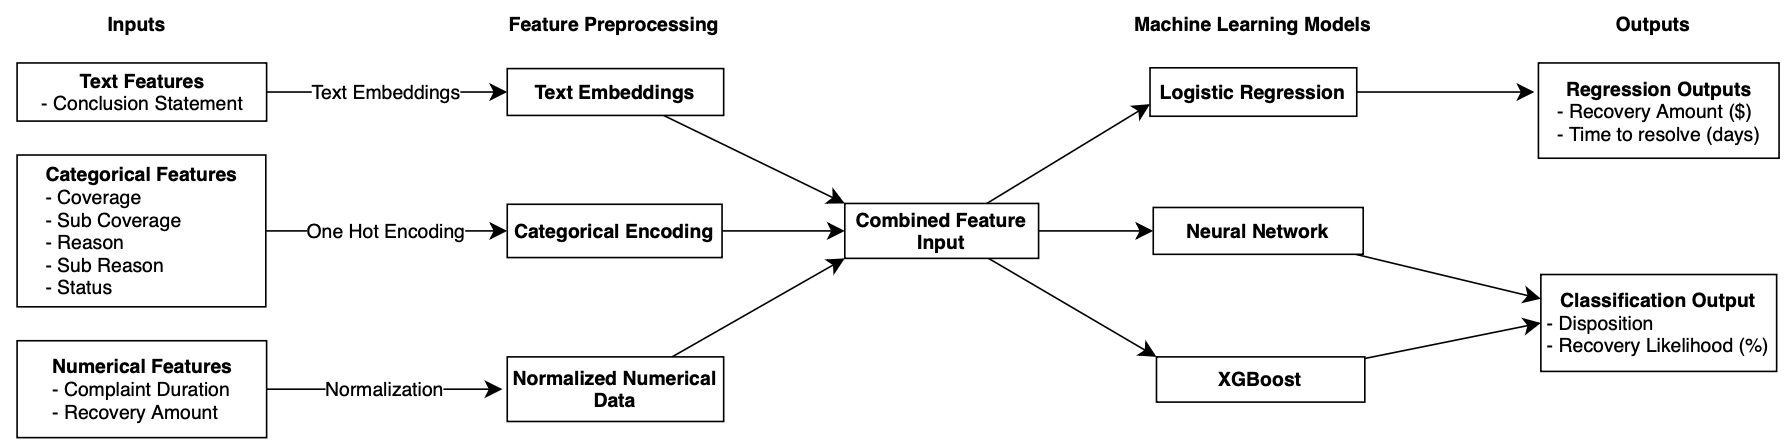
\includegraphics[width=1.0\textwidth]{ml-flowchart.png}
  \caption{Pipeline}
  \label{fig: Pipeline}
\end{figure}

\section{Dataset}

\subsection{Data Source}
“Insurance Company Complaints” dataset from Kaggle. Public dataset of consumer complaints filed in Connecticut.

\subsection{Dimensions}
\begin{itemize}
  \item 32,267 rows, 12 columns
\end{itemize}

\subsection{Data Preprocessing}
\begin{itemize}
  \item Impute incomplete rows/columns
  \item Derived features:
  \begin{itemize}
    \item Complaint duration: Days between 'Closed' and 'Opened'
    \item Text embeddings
  \end{itemize}
  \item Normalize numerical features
  \item Encode categorical variables (one-hot)
\end{itemize}

\subsection{Embedding Strategy}
Pre-trained embeddings (Word2Vec, GloVe) to represent text features semantically.

\section{Experimental Evaluation}

\subsection{Evaluation Methodology}

To assess the performance of our models, we used a combination of loss metrics, classification reports, and confusion matrices. These tools provide both high-level and granular insights into how well the models performed on the classification task.

The classification report includes standard performance metrics such as accuracy, precision, recall, and F1-score. Accuracy provides an overall measure of model correctness, while precision and recall offer a deeper understanding of the model’s behavior in distinguishing between specific classes — particularly in identifying false positives and false negatives. The confusion matrix further supports this analysis by visually representing the distribution of predicted versus actual labels.

As a starting point, we implemented two models of varying complexity: logistic regression & random forest. These models served as a baseline for comparison. Logistic regression was chosen because it is a simple, interpretable model that provides a useful reference point. While it lacks the complexity and capacity of more advanced models like neural networks and decision trees, its performance establishes a lower bound against which improvements from more sophisticated models can be measured. 

This model performance can be compared to the random forest classification model, which is slightly more sophisticated and complex. Comparing the results from these two models tells us if our data benefits from a more complex model, and gives us insights into the dataset.

\subsection{Results}
\begin{enumerate}
  \item Logistic Regression (baseline)
  \begin{itemize}
    \item accuracy: 0.34
  \end{itemize}
  This metric suggests the model is not performing very well. This is expected, as a logistic regression model is much too simple to capture the fine details and correlations in the data.
  \begin{itemize}
    \item Low F-1 score for smaller categories, and High F-1 score for large categories.
  \end{itemize}
  This shows that the model rarely makes correct predictions for classes with fewer samples, and the high recall indicates there are many false positives in the classifications. This is reflected in the low F-1 score for these classes.
  \item Random Forest
  \begin{itemize}
    \item accuracy: 0.60
  \end{itemize}
  This metric shows a significant improvement over the Logistic Regression model, which indicates that the data benefits from a higher degree of model complexity.
  \begin{itemize}
    \item Low F-1 score for smaller categories, and High F-1 score for large categories.
  \end{itemize}
  This trend continues from the Logistic Regression Model, suggesting that the models are likely not predicting the disposition correctly, but rather are classifying most data points into the most common category, giving the illusion of correct predictions.

  This indicates problems that need to be addressed in training more complex models. One techniques considered is using SMOTE (Synthetic Minority Over-Sampling Technique) to helpe combat the class imbalance in the dataset.
  \item Nueral Network
  NN accuracy is 71\% and loss is .86. So accuracy seems okay but we have a lot of loss. This tells us that our neural network can’t  generalize well and is overfit. 
  Our data is a little tricky in where there’s a lot of classes, some are not so important (noise), so if we wanted to reduce loss more, getting rid of less important classes would probably do the trick.
  Most of the gain’s in performance for our neural network (and our models in general) would probably come from feature engineering. 
\end{enumerate}

\subsection{Discussion}
Our initial experimentation with baseline models of Linear Regression and Random Forest Classification show two main things:
\begin{itemize}
  \item The data benefits from a more complex model to capture fine details and correlations between features.
  \item The data is severly imbalanced, with a few categories dominating the dataset, which is an issue that needs to be addressed when training subsequent models.
\end{itemize} 

\section{Conclusion}
Our study demonstrates the potential for creating a suitable model for insurance complaint data. Our models that we created shows that we can predict the disposition (the resolution of the complaint) with decent accuracy (60-70\%). We compared more complex models (XGBoost, Random Forest, Neural Network) to a simpler logistic regression model to prove a model for this data would benefit from having more complexity. We also learned the limitations of our data, namely: unbalanced classes, and incomplete data rows. Through trial and error we learned that most significant performance gains would be made in feature engineering our data set in order to make our model’s generalize better. Our paper proves the value in using machine learning techniques to predict user insurance data complaint resolutions. 

\bibliographystyle{plainnat}
\bibliography{references}

% Add actual entries to references.bib or inline here
% Example inline references:
\begin{thebibliography}{9}

\bibitem{johnson2023}
Johnson, M., Albizri, A., \& Harfouche, A. (2023).
Responsible Artificial Intelligence in Healthcare: Predicting and Preventing Insurance Claim Denials.
\textit{Information Systems Frontiers}, 25, 2179–2195. \url{https://doi.org/10.1007/s10796-021-10137-5}

\bibitem{gilpin2018}
Gilpin, L. H., Bau, D., Yuan, B. Z., Bajwa, A., Specter, M., \& Kagal, L. (2018).
Explaining explanations: An approach to evaluating interpretability of machine learning.

\end{thebibliography}

\end{document}